\documentclass[conference]{IEEEtran}
\IEEEoverridecommandlockouts
\usepackage{cite}
\usepackage{amsmath,amssymb,amsfonts}
\usepackage{graphicx}
\usepackage{booktabs}
\usepackage{xcolor}
\usepackage{url}
\usepackage{hyperref}
\usepackage{tikz}
\usetikzlibrary{positioning,arrows.meta}
\newcommand{\todo}[1]{\textcolor{red}{[TODO: #1]}}
% generated tables shrink to the column (or page) width only when they are wider than it
\newcommand{\fittable}[1]{\resizebox{\ifdim\width>\linewidth\linewidth\else\width\fi}{!}{#1}}

% Every number in this paper is generated from results/ by scripts/make_tables.py and
% scripts/make_xai_numbers.py (bash scripts/run_experiments.sh xai). No value is typed by hand.
\input{generated/numbers}
\input{generated/numbers_xai}

\begin{document}

\title{PROVEX: Faithful, Tiered Explanations of\\Provenance-Based Intrusion Alerts for SOC Analysts}

\author{\IEEEauthorblockN{Devang Dhanuka}
\IEEEauthorblockA{\textit{Department of Software Engineering} \\
\textit{Rochester Institute of Technology}\\
Rochester, NY \\
dd9098@rit.edu}
\and
\IEEEauthorblockN{Nidhi Rastogi}
\IEEEauthorblockA{\textit{Department of Software Engineering} \\
\textit{Rochester Institute of Technology}\\
Rochester, NY \\
nxrvse@rit.edu}
}

\maketitle

\begin{abstract}
Security operations centres increasingly receive alerts from learned provenance-based intrusion
detectors, but such an alert says only that activity is improbable. Analysts accept explanations
readily, so an explanation that does not reflect what drove an alert is a safety risk. We study what a
faithful explanation can tell an analyst, using KAIROS on DARPA TC E3 CADETS and organising the study
around NIST's four principles of explainable AI. We rebuild KAIROS exactly from upstream; it detects
\NumAttacksDetected{} of the four attacks, and \FracPriorEvents{} of the events in its alerts are
anomalous from the action type alone. We present PROVEX, a tiered explanation layer. Its Tier-1 alert
story reduces the two alerts from \FlaggedEventsSix{} and \FlaggedEventsTwelve{} flagged events to
\StoryItemsSix{} and \StoryItemsTwelve{} actions, puts an attacker action first in both, and lets a
simulated analyst cut the windows to escalate from \TriageWindowsBefore{} to \TriageWindowsAfter{}
without missing an attack window. Deletion tests on an exact replay show that rare-action alerts have no
causal subgraph (a random subgraph passes the usual sufficiency test), that context-dependent alerts are
explained faithfully by a plain gradient, and that GNNExplainer, GraphMask and attention are no better
than random once removing an event means deleting it. PROVEX's history-gated explainers, its most
expensive component, add no faithfulness: KAIROS's memory is nearly empty, and the evidence lies in recent
neighbour edges. We close with implications for XAI in SOC operations.\end{abstract}

\begin{IEEEkeywords}
Explainable AI, security operations, provenance, intrusion detection, temporal graph networks
\end{IEEEkeywords}

%=====================================================================================================
\section{Introduction}
\label{sec:intro}
Security operations centres (SOCs) receive far more alerts than they can investigate. Most of the alarms
analysts call false positives are true detections of benign triggers, and validating them is tedious work
that can lead to burnout~\cite{alahmadi}. Provenance-based intrusion detection systems (PIDS) promise better alarms: they
represent system activity as a graph of processes, files and sockets and learn what normal activity looks
like~\cite{kairos,unicorn,orthrus,bilot}. A learned detector's alert, however, says only \emph{that}
activity is improbable under its model, not \emph{why}. Practitioners ask for the evidence behind a score,
for context about the event, and for concise output~\cite{mink,dong}; industrial teams budget fewer than 50
nodes per alarm graph~\cite{dong}.

Explanations help only if they are right. In a survey of 248 SOC analysts and 24 interviews,
analysts accepted explanation output readily, even from less accurate models, when it looked relevant
and backed by evidence~\cite{tmt}. An explanation that is plausible but does not reflect what drove the
alert can therefore steer an analyst wrongly. For SOC use, faithfulness is a safety property. NIST's
principles of explainable AI make the same demand (\emph{explanation accuracy}) and add a second one:
a system should say where its knowledge ends~\cite{nist}.

This paper asks what a faithful explanation of a learned provenance detector can tell an analyst, and how
much it reduces the work of deciding on an alert. We study KAIROS~\cite{kairos}, a representative
detector built on a temporal graph network (TGN)~\cite{tgn} with public code, on DARPA TC Engagement~3
CADETS~\cite{darpa}. We organise the study around NIST's four principles (explanation, meaningful,
explanation accuracy, knowledge limits)~\cite{nist} and the distinctions between transparency,
interpretability and explainability drawn in the XAI literature~\cite{lipton,arrieta}, which we use
operationally (\S\ref{sec:background}). Our evaluation is \emph{functionally
grounded}~\cite{doshivelez}: we run no user study, and instead measure proxies for an analyst's work
(items to read, the rank of the first attacker action, and a simulated analyst that decides from the
explanation alone) against two separately produced encodings of DARPA's ground truth: node labels from
ORTHRUS/PIDSMaker~\cite{orthrus,bilot}, and the attack steps in DARPA's ground-truth report~\cite{darpa},
which we encode ourselves as observable entity patterns.

\textbf{Findings.} \emph{Transparency:} our replay reproduces KAIROS's scores exactly
(\ParityDaysOK{} days), and the rebuilt detector catches \NumAttacksDetected{} of the four attacks.
\emph{Interpretability:} \FracPriorEvents{} of the events in KAIROS's alerts exceed the threshold from the
event type alone, context reaches the score only through neighbours' messages, and the two missed attacks
are a cost of aggregating windows into queues. \emph{Explanation and meaningfulness:} a Tier-1 story cuts
an alert from thousands of events to tens of actions and, ordered by novelty rather than score, puts the
attacker first; a simulated analyst escalates \TriageWindowsAfter{} of \TriageWindowsBefore{} alerted
windows and misses none with attacker activity. \emph{Explanation accuracy:} for rare-action alerts no
subgraph is a cause and any subgraph passes a sufficiency test; for context-dependent alerts a gradient is
as faithful as search-based explainers, while standard GNN explainers fail exact deletion and
GNNExplainer's standard objective explains why the event looks normal; explanations over memory history add cost but no
faithfulness, because the memory is nearly empty. \emph{Knowledge limits:} the variational explainer's
uncertainty is calibrated (ECE \CalECE{}), context-dependent alerts are marginal, PROVEX's deletions agree
with a full re-execution of the detector on the alert decision in \EsevenFlipAgree{} of cases, and the
detector's blind spot for short attacks has to be reported alongside its explanations.
\textbf{Contributions.}
\begin{itemize}
\item \textbf{Transparency} (\S\ref{sec:transparency}). An exact, auditable reproduction of KAIROS from
  upstream, whose replay matches the detector's scores on every test day, and an account of the data as
  the detector sees it, including label errors in the public ground truth.
\item \textbf{Interpretability} (\S\ref{sec:interpretability}). A global account of what KAIROS relies on:
  which channel carries an alert, how much of an alert is the event type alone, and why two of the four
  attacks raise no alert.
\item \textbf{PROVEX} (\S\ref{sec:provex}), a tiered explanation layer that follows analysts' stated
  needs~\cite{tmt}: a Tier-1 alert story for triage, Tier-2 anomaly-faithful explanations of
  individual events over neighbour edges and history, and Tier-3 internals with uncertainty and limits.
\item \textbf{A principle-organised evaluation} (\S\ref{sec:eval}): decision burden, faithfulness by alert
  class, story versus DARPA's account of each attack, knowledge limits and cost.
\item \textbf{Implications for XAI in SOC operations} (\S\ref{sec:implications}).
\end{itemize}
Code, patches to upstream KAIROS, models and all outputs are released.

%=====================================================================================================
\section{Background and Related Work}
\label{sec:background}
\subsection{How KAIROS scores and alerts}
A day of audit data is a time-ordered stream of events $e_k=(u_k,v_k,y_k,t_k,\mathbf{r}_k)$. Here
$u_k,v_k$ are entities, $y_k$ is one of seven event types, and $\mathbf{r}_k$ is a raw message of hashed
endpoint features plus a one-hot type. KAIROS processes the stream in batches of $B{=}1024$. For a batch,
a last-neighbour loader gives every endpoint its $K$ most recent interactions as in-edges. A two-layer
TransformerConv embeds the endpoints; its inputs are TGN memory states $\mathbf{s}$, and its edge features
are a cosine time encoding concatenated with the raw message. An MLP predicts the type distribution
$p(y\mid e)$, and the anomaly score is $L(e)=-\log p(y_e\mid e)$. Only after scoring does memory update:
each node aggregates the \emph{latest} message of the batch and applies a GRU. Memory and loader reset at
the start of each day.

Windows close at batch boundaries once 15~minutes have elapsed. Events with $L>\tau_w$, where
$\tau_w=\mu_w+1.5\sigma_w$ over the window, are anomalous. Windows that share rare anomalous entities are
chained into queues, and a queue whose score exceeds a threshold $\beta$ raises an alert on all its
windows~\cite{kairos}. The released code scores a queue as $\prod_w(1+\bar L_w)$ over its windows' mean
anomalous scores and sets $\beta{=}100$; we use it unchanged. For investigation, KAIROS builds a weighted
graph from the anomalous edges of the alerted windows and splits it with Louvain community detection; each
community is a candidate \emph{summary graph}.

\subsection{Principles of explainability}
Lipton separates transparency (whether a person can simulate a model, understand its parts or its
training algorithm) from post-hoc interpretability, such as local explanations of individual predictions,
and warns that post-hoc accounts can mislead~\cite{lipton}. Barredo Arrieta et~al.\ distinguish
interpretability, a passive property of a model that they also call transparency, from explainability,
the active account a model gives of its functioning~\cite{arrieta}. A learned PIDS cannot be made
simulatable, so we use the three terms operationally: \emph{transparency} means the detector can be
inspected and re-run exactly, so that every alert can be re-derived; \emph{interpretability} means its
global behaviour maps to concepts an analyst understands; and \emph{explainability} means a specific
alert comes with an account of why. NIST's four
principles~\cite{nist} state what an explainable system owes its users: it delivers evidence or reasons
for its outputs (\emph{explanation}); these are understandable to their intended consumers
(\emph{meaningful}); they correctly reflect the reason for the output (\emph{explanation accuracy});
and the system operates only under the conditions it was designed for and when it reaches sufficient
confidence in its output, declaring the cases where its answers are not reliable (\emph{knowledge limits}). Doshi-Velez and Kim~\cite{doshivelez} distinguish application-grounded,
human-grounded and functionally grounded evaluation; the last uses formal proxies and no humans, and is
what this paper does.

\subsection{What SOC analysts need}
Interviews and surveys agree on a small set of needs. Analysts want actionable indicators, the evidence
behind a score, narratives over time and concise output, and needs differ by role: Tier-1 analysts want
terse summaries and indicators, Tier-2 analysts causal narratives, and Tier-3 analysts internals,
uncertainty and behaviour over time; progressive disclosure serves all three~\cite{tmt}. Practitioners
also want links to earlier events and worry about overload and misleading explanations~\cite{mink}.
Good alarms are reliable, explainable, analytical, contextual and transferable~\cite{alahmadi}. In an
operational pilot, XAI features were rarely used and did not improve decisions~\cite{nyreyu}, and only
14\% of XAI-for-security papers run a user study~\cite{nadeem}.

\subsection{Explaining graph-based detectors}
GNNExplainer~\cite{gnnexplainer} learns soft edge masks; GraphMask~\cite{graphmask} learns amortised
hard-concrete gates; PGExplainer~\cite{pgexplainer} amortises mask prediction; CF-GNNExplainer~\cite{cfgnnexplainer}
learns minimal deletions that flip a prediction. For temporal graphs, T-GNNExplainer~\cite{tgnnexplainer}
searches subsets of past events and TempME~\cite{tempme} explains with temporal motifs; only recent
methods attribute through TGN memory~\cite{memexplainer,xiong}. All of them explain a model's prediction (a
class or a link probability), not an anomaly score defined as the loss of an observed outcome, which is
what KAIROS alerts on. For provenance detectors, ProvExplainer~\cite{provexplainer} distils
a GNN detector into an interpretable decision-tree surrogate and ProvX~\cite{provx} searches counterfactual perturbations;
NoDoze~\cite{nodoze} ranks alerts by the rarity of their causal graphs, and ORTHRUS~\cite{orthrus} frames
the analyst effort a detector's output costs as quality of attribution, measured by the flagged nodes an
analyst must inspect. Evaluation pitfalls are well documented: saliency methods can be
insensitive to the model~\cite{adebayo}, removal-based scores need care~\cite{hooker}, security work needs
its own evaluation criteria~\cite{warnecke,arp}, and benchmark choices change conclusions about PIDS~\cite{bilot,guerra}.
%=====================================================================================================
\section{Study Design}
\label{sec:design}
Table~\ref{tab:hypotheses} maps our hypotheses to the principles. H1 asks whether an explanation reduces
the burden of deciding on an alert; H2 whether the story it tells is the detector's; H3 whether that story
matches the attack; H4 whether limits are visible; H5 what it costs.

\begin{table*}[t]
\centering\small
\caption{Hypotheses, the principles they test, and how we measure them (functionally grounded).}
\label{tab:hypotheses}
\begin{tabular}{p{0.20\textwidth}p{0.16\textwidth}p{0.32\textwidth}p{0.21\textwidth}}
\toprule
Hypothesis & Principle & Measure & Ground truth / baseline\\
\midrule
H1: an explanation reduces the decision burden of an alert & Meaningful; decision support & items to read; rank of the first attacker action; simulated analyst deciding per window from the explanation only; a novelty-only control & raw KAIROS alert; KAIROS summary graphs; DARPA indicators\\
H2: the story is the detector's story & Explanation accuracy & deletion and insertion tests per alert class; minimal counterfactual size; exact replay & every item's effect, by exact deletion\\
H3: the story matches the attack & Accuracy; meaningful & DARPA attack steps recovered; size against a 50-node budget & DARPA report; ORTHRUS labels\\
H4: limits are visible & Knowledge limits & uncertainty calibration; stability; approximation flags; detector blind spots & exact posteriors; full re-execution\\
H5: cost fits the tier & Explanation & time per alert event and per tier & --\\
\bottomrule
\end{tabular}
\end{table*}

\textbf{Data, detector and splits.} We use the CADETS~E3 day graphs for 2018-04-02 to 04-13 and its four
attacks (04-06, 04-11, 04-12 and 04-13). KAIROS is rebuilt from upstream at a pinned commit with
documented patches (seeds, all test days, all four attacks, PyG~2.7 compatibility), trained on 04-02 to
04-04 with \NumSeeds{} seeds and the upstream hyper-parameters. Days 04-03 to 04-05 initialise the
rare-node scores of the queues, 04-05 is the validation day and 04-06 to 04-13 are test days.

\textbf{Ground truth.} Node labels come from ORTHRUS/PIDSMaker~\cite{orthrus,bilot}, mapped to KAIROS
nodes by name, which is how KAIROS keys them. ORTHRUS's authors derived these labels from DARPA's textual
report; we encode the same report a second way, as each attack's steps~\cite{darpa} (exploit, staging, payload, privilege elevation and command and control, reconnaissance, lateral
payload, injection) as patterns over IP addresses, file paths and process names, with the report's times
and 15~minutes of slack.

\textbf{What is explained.} PROVEX explains the alerts KAIROS raises, true and false positives alike.
Within each alerted window we take the top \TopN{} anomalous events by score plus a uniform sample of
\SampleN{} more (\NumAlertEvents{} alert events in total). For the comparison of techniques we use every
context-dependent alert event and a stratified sample of the rest (\S\ref{sec:eval}).

%=====================================================================================================
\section{Transparency: An Exact, Auditable KAIROS}
\label{sec:transparency}
\input{generated/tab_detection}
Transparency for a SOC means that the alert can be re-derived: given the model, the data and the
configuration, anyone obtains the same scores. PROVEX re-executes KAIROS with the same batch partition,
per-day resets, window boundaries and per-event losses; the replay matches the detector's own window
files on \ParityDaysOK{} days. Replay runs on CPU, because GPU scatter kernels break ties
nondeterministically. Every reported item is keyed by its absolute event index and global node
identifiers, so an explanation can be audited against the raw data.

\textbf{Detection.} Under its own alert rule KAIROS detects \NumAttacksDetected{} of the four attacks
(\AttacksDetected{}; Table~\ref{tab:detection}), identically in all seeds. Upstream evaluates only 04-06
and 04-07; on all eight test days most alerted windows are not attack windows.

\textbf{The data as the detector sees it.} The graph has \NumNodes{} nodes: \NumFiles{} files,
\NumNetflows{} sockets and only \NumProcesses{} processes, because KAIROS keys processes by name, so
every \texttt{nginx} process is one node. Test days have \EventsPerTestDay{} million events. The
recording has gaps of \GapSixMin{} minutes on 04-06 and \GapElevenMin{} on 04-11 (DARPA notes host
crashes), and 04-13 appears truncated: \ActiveFilesThirteen{} active files, against
\ActiveFilesOtherTest{} on the other test days.

\textbf{The public labels have errors.} The ORTHRUS labels for 04-06 omit the attacker's shellcode server
(78.205.235.65), its second payload server (152.111.159.139) and the payload written to
\texttt{/var/log/devc}, all of which DARPA's report names. The 04-13 labels include a benign wget mirror
of \texttt{/usr/home/user/eraseme} through a name collision with the attacker's \texttt{eraseme}. A
phishing relay that DARPA ran through CADETS' mail server is not labelled at all. We therefore report
DARPA's steps alongside the labels.

%=====================================================================================================
\section{Interpretability: What KAIROS Relies On}
\label{sec:interpretability}
Before explaining single alerts we ask what drives them globally. For each alert event we compute its
score under six interventions: unchanged; all neighbour edges removed; history removed; both removed;
the memory of the event's two endpoints zeroed; and the type prior alone (no edges, zero memory).

\textbf{Context reaches the score only through neighbours.} Removing every neighbour edge gives exactly
the type-prior score, and zeroing the memory of the event's own endpoints changes the score by at most
\MemZeroMaxEffect{} (10th to 90th percentile). The reason is that the memory is nearly empty: over
\MemPathN{} alert events of 04-12, the endpoints' memory vectors have a median norm of \MemPathMemNormU{},
the memories of the other nodes in the computation graph a median of \MemPathNodesNorm{} (at most
\MemPathNodesNormMax{}), and the term through which an endpoint's own memory enters the first layer moves
that layer's output by a median of \MemPathSkipNormU{} against an output norm of \MemPathConvNormU{}.
What reaches the score is the attention-weighted messages of recent neighbour edges, and with memory this
small their content must come mainly from the edges' own features: event type, endpoint hashes and timing.

\textbf{Most alerts are about the action itself.} Of the \NumAlertEvents{} alert events,
\NumPriorEvents{} (\FracPriorEvents{}) exceed their window's threshold from the event type alone,
including all \NumTopRankedPrior{} of the \NumTopRanked{} top-ranked: socket receives (\NumAlertRecv{}),
writes (\NumAlertWrite{}), executions (\NumAlertExecute{}) and sends (\NumAlertSend{}). These types are
rare in CADETS, where reads, opens and closes dominate, so the model scores them as improbable almost
regardless of context. Context still moves the score (it raises it for \FracContextRaises{} of events,
by a median of \ContextGainMedianPrior{} nats), and the rank correlation between the full score and the
type prior is only \SpearmanFullPrior{}. The remaining \NumWindowEvents{} events are
\emph{context-dependent}: opens (\NumAlertOpen{}) and closes (\NumAlertClose{}) of files such as
\texttt{/etc/pwd.db} that are anomalous only because of what happened around them; removing their
neighbour edges clears the alert. No alert event depends on memory older than the explained history.

\textbf{A learned average message comes close.} GraphMask, trained to keep the score within 5\% with as
few neighbour edges as possible, replaces every edge with a learned baseline message and changes the
score by \GMAllClosedDev{} on average; its selected gates keep \GMOpenFrac{} of edges open.

\input{generated/tab_alert_rule}
\textbf{Why two attacks raise no alert.} No single window separates attack from benign activity: each
attack's best window scores at most as high as the busiest validation window (\ValMaxWindowScore{},
Table~\ref{tab:alert-rule}). Detection therefore rests on chaining windows. The 04-06 and 04-12 attacks
produce long queues ($\beta$ needed: \BetaNeededSix{} and \BetaNeededTwelve{}); 04-11 and 04-13 produce
short ones (\BetaNeededEleven{} and \BetaNeededThirteen{}). Lowering $\beta$ to 30 would catch 04-13 at
the price of \FPWindowsBetaThirty{} false-positive windows; catching 04-11 needs $\beta{=}5$ and costs
\FPWindowsBetaFive{} false-positive test windows and \ValFPWindowsBetaFive{} on the validation day.

\textbf{Benign windows ride along.} The alert rule raises every window of a queue. \NumRiderWindowsNoIOC{}
of the \NumRiderWindows{} alerted windows outside the labelled attack windows contain no event touching
DARPA's indicators; they are routine activity of \texttt{imapd}, \texttt{lsof}, \texttt{vmstat} and a
wget mirror. Inside labelled attack windows, \GTWindowIOCShare{} of anomalous events touch an indicator.
%=====================================================================================================
\section{PROVEX: Tiered Explanations}
\label{sec:provex}
\begin{figure*}[t]
\centering
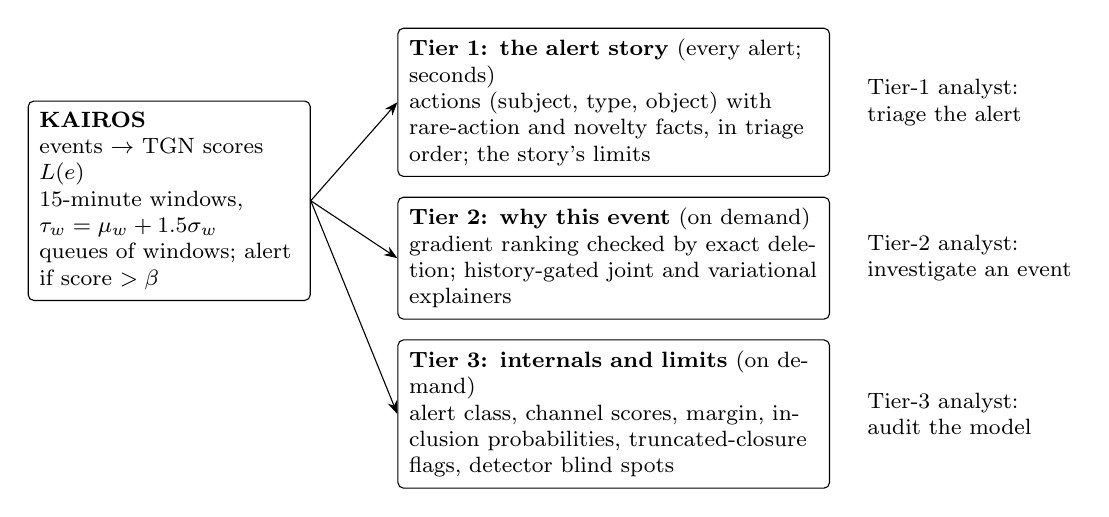
\begin{tikzpicture}[font=\footnotesize, >=Stealth, node distance=0.25cm,
    box/.style={draw, rounded corners=2pt, align=left, inner sep=4pt, text width=#1}, box/.default=5.2cm]
  \node[box=3.3cm] (k) {\textbf{KAIROS}\\ events $\rightarrow$ TGN scores $L(e)$\\ 15-minute windows, $\tau_w=\mu_w+1.5\sigma_w$\\ queues of windows; alert if score $>\beta$};
  \node[box, right=1.1cm of k, yshift=1.25cm] (t1) {\textbf{Tier 1: the alert story} (every alert; seconds)\\ actions (subject, type, object) with rare-action and novelty facts, in triage order; the story's limits};
  \node[box, below=of t1] (t2) {\textbf{Tier 2: why this event} (on demand)\\ gradient ranking checked by exact deletion; history-gated joint and variational explainers};
  \node[box, below=of t2] (t3) {\textbf{Tier 3: internals and limits} (on demand)\\ alert class, channel scores, margin, inclusion probabilities, truncated-closure flags, detector blind spots};
  \node[right=0.35cm of t1, align=left] {Tier-1 analyst:\\ triage the alert};
  \node[right=0.35cm of t2, align=left] {Tier-2 analyst:\\ investigate an event};
  \node[right=0.35cm of t3, align=left] {Tier-3 analyst:\\ audit the model};
  \draw[->] (k.east) -- (t1.west);
  \draw[->] (k.east) -- (t2.west);
  \draw[->] (k.east) -- (t3.west);
\end{tikzpicture}
\caption{PROVEX turns each KAIROS alert into three tiers of explanation, matching the analyst roles
of~\cite{tmt}. Every explanation is computed on an exact replay of the detector, and every claim about
removing an event is checked by deleting it from an exact replay of the detector.}
\label{fig:tiers}
\end{figure*}
PROVEX's tiers are informed by the roles analysts describe~\cite{tmt} (Fig.~\ref{fig:tiers}). Tier~1 is a
short story per alert for triage; Tier~2 explains individual events on demand; Tier~3 exposes internals,
uncertainty and limits. Tier-1 and Tier-3 content match what those analysts asked for. Tier-2 analysts
asked for causal narratives that link alerts across stages, which per-event explanations only begin to
provide.

\subsection{Tier 1: the alert story}
For each alert (a KAIROS queue) and each of its windows, PROVEX groups the anomalous events into
\emph{actions} (subject, event type, object), merging entities an analyst cannot tell apart (KAIROS keeps
one socket node per local and remote endpoint but labels it by the remote address). Each action carries
facts an analyst can act on: whether it is a \emph{rare action} (anomalous from its type alone, the
\FracPriorEvents{} case of \S\ref{sec:interpretability}); whether an entity is new today or was never seen
in training; whether a peer is outside the monitored network and its IP address is new today; and whether
a program new today is running. Actions are listed in a fixed triage order: new external IP addresses
first, then new programs, then score. At most 5 actions per window and 10 per alert are shown. The story
ends with its limits: rare actions are anomalous for the model from the action alone, and short attacks
can pass without any alert.

\subsection{Tier 2: what made this event anomalous}
\label{sec:objectives}
Let $\mathcal{I}(e)$ be the \emph{items} that can influence $L(e)$: the neighbour edges of the event's
two-hop computation graph and the past events inside a history window that updated the memory of the
endpoints or of entities that later fed them. An explanation scores items. We write $L(\mathbf{g})$ for
the score when item $i$ is kept with gate $g_i\in[0,1]$, so that $L(\mathbf{1})=L(e)$.

\textbf{Explain the anomaly, not the label.} GNNExplainer-style methods minimise
$\mathrm{CE}(f(G\odot\mathbf m), y_e)$. For a classifier this finds evidence \emph{for} the predicted
label. For an anomaly score $L=-\log p(y_e)$ it finds the items whose presence makes the observed type
\emph{likely}: the evidence that the event is normal. We define two
objectives with margin $\delta$ and temperature $T$:
\begin{align}
\text{preserve:}\quad &\min_{\mathbf g}\ \textstyle\sum_i g_i \ \ \text{s.t.}\ L(\mathbf g)\ge\min(L(\mathbf 1),\tau+\delta),\\
\text{counterfactual:}\quad &\min_{\mathbf g}\ \textstyle\sum_i (1-g_i) \ \ \text{s.t.}\ L(\mathbf g)\le\tau-\delta.
\end{align}
Preserve gives a minimal set of past events sufficient to sustain the alert; counterfactual gives a
minimal set whose absence would have prevented it. We relax the constraints with
$T\,\mathrm{softplus}(\cdot/T)$, which keeps gradients alive where a hinge would be flat, and work in
loss space, because the gradient of $-\log(1-p)$ vanishes for $p\approx10^{-11}$.

\textbf{Alert classes.} An alert event is \emph{window-explainable} (context-dependent) if removing all
its items brings it below the threshold, \emph{prior-driven} if not and the type prior alone exceeds the
threshold, and \emph{long-memory} otherwise. For prior-driven events no set of items is a cause, and
Tier~1's ``rare action'' is the faithful explanation.

\label{sec:history}
\textbf{History gating.} To let a gate on a past event approximate ``this event never happened'', PROVEX
replays the TGN memory update differentiably for the endpoints and their \emph{influence closure} (nodes
whose earlier messages reached them, capped at 64 and flagged when truncated). For a node with candidate
messages ordered as PyG resolves ties, gates $g_k$ give weights $w_k=g_k\prod_{j<k}(1-g_j)$ and update
probability $P=1-\prod_k(1-g_k)$, and
\[
\mathbf s_i'=P\,\frac{\sum_k w_k\,\mathrm{GRU}(\mathbf m_k,\mathbf s_i)}{\sum_k w_k}+(1-P)\,\mathbf s_i .
\]
With binary gates this is exactly the detector's update for every node in the closure: deleting the latest
message promotes the next, and deleting all of a node's messages leaves it un-updated. Two things are not
replayed: nodes outside a truncated closure keep their recorded memory, and the neighbour loader is not
back-filled with older neighbours after a deletion. We measure the resulting gap against a full
re-execution of the detector without the deleted events (E7, \S\ref{sec:eval}). Timestamps are subtracted in 64-bit integers
before conversion, since KAIROS encodes time as $\cos(\mathbf w\,\Delta t)$ with $\Delta t\sim10^{12}$\,ns.
Neighbour edges are deleted exactly by rescaling surviving messages by the attention mass that remains
at their target; PyG's explanation hook scales after the softmax and is not a deletion.

\label{sec:variational}
\textbf{Explainers.} The \emph{joint} explainer places hard-concrete gates~\cite{louizos} on all items,
minimises expected $L_0$ under the preserve or counterfactual constraint with a persistent Lagrange
multiplier, checks the result by exact deletion and repairs it greedily if needed. The \emph{variational}
explainer places a Gaussian posterior on gate logits with a temporal prior
$\mathcal N(a-\kappa\log(1+\Delta t_k/60\text{s}),1)$ and the likelihood $\sigma((L(\mathbf m)-\tau)/T)$
that the alert holds; it exports per-item inclusion probabilities, which we check against exact
posteriors by enumeration. \label{sec:graphmask}\emph{GraphMask-TC} is a faithful GraphMask for
TransformerConv: amortised gates read query, key, value and the edge's role for the explained event, and
a gated-off edge is replaced by learned baselines with the softmax recomputed. It introspects the
neighbour channel only.

\textbf{Baselines.} Random, recency, attention, gradient, integrated gradients and occlusion (over the
200 items with the largest gradient); GNNExplainer with our objective; GNNExplainer with its standard
objective (cross-entropy of the observed type) as a counter-example; and a T-GNNExplainer-style Monte-Carlo tree search over subsets of at
most 10 items, with a gradient prior in place of its learned navigator.

\subsection{Tier 3: internals and limits}
For each event, Tier~3 reports the alert class, the six intervention scores of
\S\ref{sec:interpretability}, the explainer's validity under exact deletion, inclusion probabilities,
and whether the history closure was truncated. For each alert it reports the share of rare actions and
how much of the window the shown actions cover.

%=====================================================================================================
\section{Evaluation}
\label{sec:eval}
We evaluate against the hypotheses of Table~\ref{tab:hypotheses}, in the order an analyst meets them:
deciding on an alert (H1), trusting its story (H2), relating it to the attack (H3), knowing its limits
(H4), and paying for it (H5).

\subsection{H1: Does the explanation reduce the decision burden?}
\input{generated/tab_h1}
An analyst facing a KAIROS alert sees thousands of anomalous events: \FlaggedEventsSix{} in the
\AlertWindowsSix{} windows of the 04-06 alert and \FlaggedEventsTwelve{} in the \AlertWindowsTwelve{}
windows of the 04-12 alert (Table~\ref{tab:h1}). KAIROS's own summary graphs condense them to
\SummaryNodesSix{} and \SummaryNodesTwelve{} nodes in \SummaryCommunitiesSix{} and
\SummaryCommunitiesTwelve{} communities. Read largest first, as their size suggests, an analyst reads
\SummaryNodesReadSix{} and \SummaryNodesReadTwelve{} nodes before the first community that holds an
attacker entity, well beyond the 50-node budget practitioners set~\cite{dong}. The Tier-1 story shows
\StoryItemsSix{} and \StoryItemsTwelve{} actions.

\textbf{Order matters more than size.} Ranked by KAIROS's own score, neither story has an attacker
action in its top ten: the highest-scoring actions are benign DNS replies to mail and monitoring
daemons, local \texttt{php-fpm} traffic, mail delivery and routine scripts,
which the model scores higher than the attacker's command-and-control. In the triage order, which puts
new external addresses and new programs first, the first action of both stories is the attacker's.

\textbf{Window triage.} A simulated Tier-1 analyst escalates a window only if its story shows a new
external IP address or a new program. Of the \TriageWindowsBefore{} alerted windows, the analyst
escalates \TriageWindowsAfter{}: \TriageTP{} with attacker activity and \TriageFP{} without, and misses
\TriageFN{}. The share of escalated windows that contain attacker activity rises from
\TriagePrecisionBefore{} to \TriagePrecisionAfter{}. The false escalation is a 04-06 window in which a
text browser fetched pages from new addresses and the mail server received spam.

\textbf{Is it the detector or the novelty?} The triage flag is a simple novelty rule, and an allowlist of
executable names and paths seen in training matches or beats several learned detectors on DARPA E3
data~\cite{guerra}. Table~\ref{tab:novelty}
therefore applies the same flag to every test window, with and without KAIROS.
The novelty flag on its own is not a detector. Applied to every one of the \CtlTestWindows{} test windows,
it flags \CtlNoveltyAllFlagged{}, of which \CtlNoveltyAllFP{} contain no attacker activity (precision
\CtlNoveltyAllPrecision{}), plus \CtlNoveltyAllVal{} windows of the attack-free validation day. It does
touch all four attacks (\CtlNoveltyAllTP{} of the \CtlGTWindows{} attack windows), including the two that
KAIROS misses: the attacker's new addresses and programs were there to see. Restricting the flag to the
events KAIROS scores as anomalous changes nothing: in every window with an action involving a new external
address or a new program, at least one such action is itself flagged, since these are rare actions for the
model. The detector and the
story are complementary. KAIROS's rarity scores and queues narrow the test windows to
\CtlKairosFlagged{} (precision \CtlKairosPrecision{}), and the story's facts narrow those to
\CtlKairosStoryFlagged{} (precision \CtlKairosStoryPrecision{}) without losing an attack window.\input{generated/tab_novelty}

\subsection{H2: Is the story the detector's story?}
We test every explanation by deletion with binary gates on the replay of \S\ref{sec:history}. In setting~A
an item's message is removed from the event's computation graph; in setting~B it is also removed from the
replayed memory history. These are exact interventions on PROVEX's replay, not full re-executions of the
detector without the event; H4 measures the difference. Every recomputed full score equals the
detector's (\HADropped{} events dropped in setting~A, \HBDropped{} in setting~B). Setting~A explains the
neighbour-edge channel only, which \S\ref{sec:interpretability} showed is the only route context takes,
and covers all \HAWinN{} context-dependent alert events and a stratified sample of \HAPriorN{}
rare-action ones (up to 8 per day and event type). Setting~B adds the last 16 batches of history for
\HBWinN{} context-dependent events.

\textbf{Rare-action alerts have no causal subgraph.} For every sampled rare-action event
(\HAPriorFloorAlerts{} of \HAPriorN{}) the score stays above the threshold with every neighbour edge
removed; the median margin is \HAPriorMargin{} nats. Deleting the top 10 items of any ranking clears
almost none of them (gradient: \HAPriorGradientFlipTen{}), and the most the top five items move the score
is a median of \HAPriorGradientDLFive{} nats. The usual sufficiency test is vacuous here: keeping only five
\emph{random} items sustains \HAPriorRandomKeepFive{} of these alerts, as many as keeping the best
method's five (\HAPriorGradientKeepFive{}). A subgraph shown to an analyst for such an alert would pass a
faithfulness check whatever it contained. The faithful explanation is Tier~1's: the action itself is rare
for this model. PROVEX's preserve explainer returns the empty set for these events (median size
\HAPriorJointOwnSize{}).

\input{generated/tab_faith_window}
\textbf{Context-dependent alerts have faithful explanations, and the cheapest is enough.} These
\HAWinN{} events exceed their thresholds by a median of only \HAWinMargin{} nats (10th to 90th
percentile \HAWinMarginLo{} to \HAWinMarginHi{}). Deleting the top 10 items of the gradient ranking
clears \HAWinGradientFlipTen{} of them, keeping only its top five sustains \HAWinGradientKeepFive{},
and its shortest clearing prefix has a median of \HAWinGradientMinCF{} items
(Table~\ref{tab:faith-window}). Integrated gradients, occlusion and the MCTS search, whose navigator we
replaced by the gradient, rank almost identically, which suggests that on this channel the score responds
nearly additively to individual neighbour events. A random ranking clears \HAWinRandomFlipTen{} at
$k{=}10$. PROVEX's joint explainer returns sets that exact deletion validates for every event
(\HAWinJointOwnValid{} preserve, \HAWinJointCFOwnValid{} counterfactual), but they are larger than the
gradient's prefixes (median \HAWinJointOwnSize{} and \HAWinJointCFOwnSize{} items), and its ranking clears
fewer alerts at $k{=}10$ (\HAWinJointFlipTen{}). The variational explainer is weaker still on deletion
(\HAWinVariationalFlipTen{}), and its value lies in the uncertainty it reports (H4).

\textbf{Standard tools fail the deletion test.} Deleting the top five items of GNNExplainer with our
objective lowers the score more than deleting five random items in only \HAWinGnnxAnomalyWinsFive{} of
events; for attention the figure is \HAWinAttentionWinsFive{} and for GraphMask \HAWinGraphMaskWinsFive{}.
Their masks are learned under other interventions: PyG scales messages after the attention softmax, and
GraphMask substitutes learned baselines. Neither is deletion, so their rankings do not predict what
removing an event does. GNNExplainer's standard objective is inverted, as \S\ref{sec:objectives} predicts: deleting its top
five items \emph{raises} the score for \HAWinGnnxVoneRaisesFive{} of events, and its own selected set
sustains the alert for only \HAWinGnnxVoneOwnValid{}.

\textbf{With history, nothing changes for the better.} Adding the last 16 batches of history raises the
items per event to a median of \HBWinItems{}, but the items that matter remain neighbour edges: none of the
gradient's top five items is a history-only event (\HBWinGradientHistFive{}), deleting its top ten clears
\HBWinGradientFlipTen{} of the \HBWinN{} alerts, and keeping its top five sustains \HBWinGradientKeepFive{}.
PROVEX's joint explainer does worse with history than without it: the history-gated version clears
\HBWinJointFlipTen{} at $k{=}10$ and returns validated sets of a median \HBWinJointOwnSize{} items, the
edges-only version \HBWinJointEdgesFlipTen{} with \HBWinJointEdgesOwnSize{} items. The variational
explainer is the only method whose top items are mostly history events (\HBWinVariationalHistFive{}), and
those items sustain the alert in only \HBWinVariationalKeepFive{} of events. With the near-empty memory of
\S\ref{sec:interpretability}, this refutes the expectation that motivated PROVEX's history gating, namely
that history explains context-dependent alerts with fewer removals than edges do. For KAIROS on CADETS the
memory history adds cost and no faithfulness.

\input{generated/tab_faith_prior}
\subsection{H3: Does the story match the attack?}
DARPA's report describes seven steps for each detected attack. The triage-ordered stories contain
actions of \StoryStepsSix{} (04-06) and \StoryStepsTwelve{} (04-12) of them within their
\StoryItemsSix{} and \StoryItemsTwelve{} actions; ordered by score, \StoryScoreStepsSix{} and
\StoryScoreStepsTwelve{}. KAIROS's summary graphs contain entities of \SummaryStepsSix{} and
\SummaryStepsTwelve{} steps, an upper bound, because graph nodes carry no time and some step patterns are
generic process names. The summary graphs are more complete; the stories are concise and put the attack
first. The stories do not contain the exploit of either attack, the payload drop and the \texttt{sshd}
injection of 04-06, or the staging downloads and port scans of 04-12; the summary graphs contain
entities of most of these steps, at \SummaryNodesSix{} and \SummaryNodesTwelve{} nodes.
\textbf{Faithful is not the same as relevant.} Tier-2 explanations explain the model, and the model's
context-dependent alerts are mostly benign housekeeping: of the \NumWindowEvents{} context-dependent alert
events, \NumWindowGTEndpoint{} have a labelled attack entity as an endpoint and \NumWindowDarpa{} touches a
DARPA indicator, against \NumPriorGTEndpoint{} and \NumPriorDarpa{} of the \NumPriorEvents{} rare-action
events. Accordingly, Tier-2 rankings rarely place other attacker entities among their top five items:
on events whose endpoint is a labelled attack entity, the gradient's precision at five is
\HAWinGradientGtPFive{} (context-dependent) and \HAPriorGradientGtPFive{} (rare-action), and no method
does markedly better. A faithful explanation of a benign context-dependent event is still useful, because it
shows the analyst \emph{why} the event can be dismissed, but it should not be mistaken for attack evidence.
\subsection{H4: Are the limits visible?}
\textbf{The variational explainer's uncertainty is calibrated.} For each context-dependent event of the
setting-B list (in setting~A) we enumerate all $2^{10}$ keep-masks over the explainer's ten most uncertain
items and compare its inclusion probabilities with the exact posterior. Over \CalPairs{} item-seed pairs the
expected calibration error is \CalECE{} (mean absolute error \CalMeanErr{}, largest \CalMaxErr{}). When
the explainer reports a 0.7 probability that an event is needed, the exact posterior under the same
prior and likelihood agrees to within a few points on average. A Tier-3 analyst can read the probabilities as
the model's own uncertainty, though not as the probability that the event is malicious.

\textbf{Stability differs sharply.} Re-run with five seeds on the same events, the variational explainer's
top five items overlap with Jaccard \StabVariationalJaccard{} (Kendall $\tau_b$
\StabVariationalKendall{}), the joint explainers' with \StabJointJaccard{} (preserve) and
\StabJointCFJaccard{} (counterfactual), and GNNExplainer's with \StabGnnxAnomalyJaccard{}. Gradient-based
rankings have no seed and are identical on every run. An analyst who asks twice and gets a different answer
from GNNExplainer has no reason to trust either.

\textbf{Approximations are flagged and measured.} In setting~B every influence closure reached the
64-node cap (exact scope in \EsevenExact{} of cases), and Tier~3 flags this. We compared PROVEX's deletions
with full re-executions of the detector without the deleted events: \EsevenN{} cases, made of the top 1, 5
and 20 items of the counterfactual explanation and random sets of the same sizes for each setting-B event.
The two agree on whether the alert survives in \EsevenFlipAgree{} of cases: in \EsevenRandomFiveAgree{} of
random deletions, which barely move the score, but only \EsevenTopOneAgree{}, \EsevenTopFiveAgree{} and
\EsevenTopTwentyAgree{} for the top 1, 5 and 20 items. Smaller deletions are understated (the top five
lower the score by a median of \EsevenTopFiveDropReplay{} nats in the replay, against
\EsevenTopFiveDropFull{} on re-execution) and larger ones overstated (\EsevenTopTwentyDropReplay{} against
\EsevenTopTwentyDropFull{} for the top twenty). The gap has two causes: the truncated closure, and the
neighbour loader, which on re-execution fills a deleted neighbour's slot with an older one. Setting~A's
edge deletions share the second cause; we did not measure them separately. Deletion claims in this paper
are therefore exact statements about an intervention on PROVEX's replay, and approximate statements about
what would have happened had the events never occurred, right on the alert decision for between
\EsevenTopFiveAgree{} and \EsevenTopOneAgree{} of deletions of top items.

\textbf{The detector's limits are part of the explanation.} Every alert story ends with the limits of
\S\ref{sec:interpretability}: rare actions are anomalous from the action alone, context-dependent alerts
are marginal (median \HAWinMargin{} nats above threshold), and short attacks can pass without any alert.
Two of the four attacks did (\MissedAttacks{}); lowering the alert threshold to catch them costs the
false-positive windows of Table~\ref{tab:beta}.
\subsection{H5: What does it cost?}
Tier~1 needs no further model computation: it groups the scores KAIROS already produced and joins them
with first-seen dates. Tier~2 needs each event's computation graph, captured by replaying the day on CPU
once for all the events explained that day. On the neighbour-edge channel a gradient takes
\HAWinGradientTime{}~s per event, integrated gradients \HAWinIntGradTime{}~s, the joint explainer
\HAWinJointTime{}~s (preserve) and \HAWinJointCFTime{}~s (counterfactual), and the variational explainer
\HAWinVariationalTime{}~s, on one CPU thread. All fourteen methods with their deletion tests take a
median of \HAWallMedian{}~s per event. With 16 batches of history the joint and variational explainers
take \HBWinJointTime{}~s and \HBWinVariationalTime{}~s per event, while a gradient over the same items takes
\HBWinGradientTime{}~s. Faithful Tier-2 rankings are therefore cheap enough to precompute for every
context-dependent alert event. Calibrated uncertainty belongs on demand, which matches the progressive
disclosure analysts ask for~\cite{tmt}, and for this detector history explanations are not worth their cost.%=====================================================================================================
\section{Case Studies}
\label{sec:cases}
\input{generated/story_4_12}
\textbf{04-12: the alert an analyst would read.} Table~\ref{tab:story-4-12} is the Tier-1 story of the
04-12 alert, which spans \AlertWindowsTwelve{} windows and \FlaggedEventsTwelve{} flagged events. Its first
actions are DARPA's command-and-control step: the Drakon implant \texttt{XIM} sending to and receiving from
53.158.101.118, both flagged as a new external address used by a program first seen that day. The second
implant follows, run as \texttt{test} and calling 192.113.144.28, and further down \texttt{XIM} is executed
from \texttt{/tmp} and the micro-APT is executed as \texttt{/var/log/sendmail}. Each of these is a rare
action for KAIROS, and none needs a subgraph to be understood. The story also shows its limits: the
exploit itself (a request to \texttt{nginx}), the staging downloads and the port scans of eight internal
hosts are not in the story, although KAIROS's summary graphs contain entities of the first two.
\input{generated/story_4_6}
\textbf{04-06.} The story of the 04-06 alert (Table~\ref{tab:story-4-6}) leads with the payload
\texttt{vUgefal} talking to its command-and-control server 139.123.0.113 and to 61.167.39.128, and with
\texttt{nginx} exchanging data with the staging server 200.36.109.214. It also contains the one window the
simulated analyst escalates wrongly, in which a text browser fetched pages from new addresses.

\textbf{04-11: the alert that never came.} KAIROS raised no alert on 04-11, so PROVEX had nothing to
explain. The attack's single window was no more anomalous than a busy benign one, and its queue scored
\BetaNeededEleven{}, far below $\beta{=}100$. An analyst relying on alerts would not have seen it, and
nothing in the explanation layer could have changed that. This is the case for reporting the detector's
blind spots alongside its explanations.
%=====================================================================================================
\section{Implications for XAI in SOC Operations}
\label{sec:implications}
\textbf{Say ``rare action'' when that is the truth.} \FracPriorEvents{} of KAIROS's alert events are
anomalous because of what kind of action they are. For them no subgraph is a cause, and any subgraph,
a random one included, passes the usual sufficiency test. A SOC tool that draws an ``explanation
subgraph'' for such an alert shows a plausible story that the detector did not use, which is exactly
the kind of output analysts are inclined to accept~\cite{tmt}. The faithful message is short: this
process did something this model rarely sees, such as writing to a socket or executing a file. It is
also what Tier-1 analysts ask for~\cite{tmt}.

\textbf{Anomaly scores are not triage priorities.} Ranked by score, the stories led with benign DNS,
mail and maintenance actions. Combining the detector's rarity signal with facts an analyst would check
anyway (is this address or program new today?) put the attacker first in both alerts. Explanations
should carry such context as first-class facts, as practitioners ask~\cite{alahmadi,mink}.
Neither half works alone: the novelty facts flag \CtlNoveltyAllFlagged{} of \CtlTestWindows{} test windows
when applied without the detector, and the detector's \CtlKairosFlagged{} alerted windows hold
\CtlKairosFP{} without attacker activity until the story's facts are added.
\textbf{Test an explanation by the intervention it claims.} The standard tools we tested failed exact
deletion because their masks implement other interventions. A silent change of model state, such as a
library call that leaves dropout switched on, can invalidate every explanation without any visible error.
An explanation system for a SOC should therefore verify, for every explanation it shows, that it reproduces
the detector's score and that its claims hold under the intervention they describe, and it should show
nothing rather than an unverified story.

\textbf{Prefer the cheapest faithful method.} For context-dependent alerts a gradient was as faithful as
search-based explainers at a fraction of their cost. Expensive explainers earn their place only where they
add something the analyst needs, such as validated sets or calibrated uncertainty, and should run on
demand (progressive disclosure~\cite{tmt}).

\textbf{Interpret before you explain.} PROVEX's most elaborate component, a differentiable replay of the
TGN memory that lets an explanation delete past events, added cost and no faithfulness, because KAIROS's
memory is nearly empty. The global checks of \S\ref{sec:interpretability} cost minutes and would have
predicted this. Before building per-event explainers for a detector, find out which of its channels
actually carry its alerts.

\textbf{Show how marginal an alert is.} Context-dependent alerts sat a median of \HAWinMargin{} nats
above their threshold, and removing a handful of past events cleared most of them. A Tier-3 view should
say so: an alert that a few small changes would clear calls for corroboration, not action.

\textbf{State what the detector cannot see.} Two of the four attacks raised no alert, so there was
nothing to explain. Silence from the detector is not evidence of safety: short attacks pass KAIROS's
aggregation, and closing that gap costs many false-positive windows (Table~\ref{tab:beta}). Knowledge
limits belong to the detector as much as to its explanations, and analysts need both.
%=====================================================================================================
\section{Limitations}
\begin{itemize}
\item \textbf{No user study.} The evaluation is functionally grounded. Items to read, ranks and a
  simulated analyst are proxies for an analyst's work, not measurements of it~\cite{doshivelez,nyreyu}.
  Such proxies are most trustworthy once human-grounded experiments have validated them~\cite{doshivelez},
  which for these explanations has not yet been done.
\item \textbf{One detector, one host, two alerts.} We study KAIROS on CADETS~E3, where KAIROS raises two
  alerts. Conclusions may not transfer to other detectors or datasets~\cite{bilot,guerra}.
\item \textbf{The triage order was chosen after reading one story.} We fixed it after reading the 04-06
  story in score order, and did not change it for 04-12, which is the cleaner test.
\item \textbf{Ground truth.} Labels are mapped by entity name and contain errors
  (\S\ref{sec:transparency}); DARPA's steps are encoded by us from a prose report. KAIROS merges entities
  that share a name, so entity-level truth is coarser than UUID-level truth.
\item \textbf{Bounded explanations.} Tier-2 explanations in the comparison use bounded budgets and a
  bounded history window; deleted events do not back-fill the neighbour loader. Truncated closures are
  flagged and measured against full re-execution.
\item \textbf{Data quality.} 04-13 appears truncated and two days have recording gaps.
\end{itemize}

\section{Conclusion}
Explaining a learned provenance detector to a SOC starts with being honest about what drives it. For
KAIROS on CADETS, most alert events are about rare actions, and their faithful explanation is a single
line; the minority that depends on context is explained faithfully by the simplest attribution, history
adds nothing because the memory is nearly empty, and standard GNN explainers are not faithful under
deletion. A short alert story ordered by novelty did more
for triage than any per-event attribution, and the detector's silence on two of four attacks is a limit
no explanation can repair. These findings rest on functional proxies, one detector and two alerts. An
application-grounded study with analysts, which tests whether such stories change decisions, is the
necessary next step.
\section*{Reproducibility}
\begin{itemize}
\item Code: \url{https://github.com/devang1304/provex}, tag \texttt{\ReleaseTag}.
\item Patches to upstream KAIROS (commit \texttt{0e0b633}) are applied by \texttt{kairos/setup\_upstream.sh}.
\item Results, models and logs are archived at \ReleaseDOI.
\item Hardware: \HardwareCPU{} for replay and explanation, and \HardwareGPU{} for training.
\item Every number and table is produced by \texttt{bash scripts/run\_experiments.sh xai} and
  \texttt{tables}.
\end{itemize}
\begin{thebibliography}{00}
\bibitem{kairos} Z.~Cheng, Q.~Lv, J.~Liang, Y.~Wang, D.~Sun, T.~Pasquier, and X.~Han, ``KAIROS: Practical intrusion detection and investigation using whole-system provenance,'' in \emph{Proc. IEEE S\&P}, 2024, pp.~3533--3551, doi:10.1109/SP54263.2024.00005. Code: \url{https://github.com/ProvenanceAnalytics/kairos}.
\bibitem{tgn} E.~Rossi, B.~Chamberlain, F.~Frasca, D.~Eynard, F.~Monti, and M.~Bronstein, ``Temporal graph networks for deep learning on dynamic graphs,'' presented at the \emph{ICML Workshop on Graph Representation Learning and Beyond (GRL+)}, 2020, arXiv:2006.10637.
\bibitem{unicorn} X.~Han, T.~Pasquier, A.~Bates, J.~Mickens, and M.~Seltzer, ``UNICORN: Runtime provenance-based detector for advanced persistent threats,'' in \emph{NDSS}, 2020, doi:10.14722/ndss.2020.24046.
\bibitem{orthrus} B.~Jiang, T.~Bilot, N.~El~Madhoun, K.~Al~Agha, A.~Zouaoui, S.~Iqbal, X.~Han, and T.~Pasquier, ``ORTHRUS: Achieving high quality of attribution in provenance-based intrusion detection systems,'' in \emph{USENIX Security}, 2025, pp.~7173--7192.
\bibitem{bilot} T.~Bilot, B.~Jiang, Z.~Li, N.~El~Madhoun, K.~Al~Agha, A.~Zouaoui, and T.~Pasquier, ``Sometimes simpler is better: A comprehensive analysis of state-of-the-art provenance-based intrusion detection systems,'' in \emph{USENIX Security}, 2025, pp.~7193--7212.
\bibitem{darpa} DARPA I2O Transparent Computing Program, ``Transparent Computing Engagement 3 data release,'' Aug. 2018, with the ground-truth report \texttt{tc\_ground\_truth\_report\_e3\_update.pdf}. \url{https://github.com/darpa-i2o/Transparent-Computing/blob/master/README-E3.md}
\bibitem{alahmadi} B.~A.~Alahmadi, L.~Axon, and I.~Martinovic, ``99\% false positives: A qualitative study of SOC analysts' perspectives on security alarms,'' in \emph{USENIX Security}, 2022, pp.~2783--2800.
\bibitem{mink} J.~Mink, H.~Benkraouda, L.~Yang, A.~Ciptadi, A.~Ahmadzadeh, D.~Votipka, and G.~Wang, ``Everybody's got ML, tell me what else you have: Practitioners' perception of ML-based security tools and explanations,'' in \emph{IEEE S\&P}, 2023, pp.~2068--2085, doi:10.1109/SP46215.2023.10179321.
\bibitem{dong} F.~Dong, S.~Li, P.~Jiang, D.~Li, H.~Wang, L.~Huang, X.~Xiao, J.~Chen, X.~Luo, Y.~Guo, and X.~Chen, ``Are we there yet? An industrial viewpoint on provenance-based endpoint detection and response tools,'' in \emph{ACM CCS}, 2023, pp.~2396--2410, doi:10.1145/3576915.3616580.
\bibitem{tmt} N.~Rastogi, S.~Pant, D.~Dhanuka, A.~Saxena, and P.~Mairal, ``Too much to trust? Measuring the security and cognitive impacts of explainability in AI-driven SOCs,'' arXiv:2503.02065v2, Jul. 2025.
\bibitem{nist} P.~J.~Phillips, C.~A.~Hahn, P.~C.~Fontana, A.~N.~Yates, K.~Greene, D.~A.~Broniatowski, and M.~A.~Przybocki, ``Four principles of explainable artificial intelligence,'' NIST, NISTIR~8312, 2021, doi:10.6028/NIST.IR.8312.
\bibitem{arrieta} A.~Barredo~Arrieta, N.~D\'iaz-Rodr\'iguez, J.~Del~Ser, A.~Bennetot, S.~Tabik, A.~Barbado, S.~Garc\'ia, S.~Gil-L\'opez, D.~Molina, R.~Benjamins, R.~Chatila, and F.~Herrera, ``Explainable artificial intelligence (XAI): Concepts, taxonomies, opportunities and challenges toward responsible AI,'' \emph{Information Fusion}, vol.~58, pp.~82--115, Jun. 2020, doi:10.1016/j.inffus.2019.12.012.
\bibitem{lipton} Z.~C.~Lipton, ``The mythos of model interpretability,'' \emph{Communications of the ACM}, vol.~61, no.~10, pp.~36--43, Oct. 2018, doi:10.1145/3233231.
\bibitem{doshivelez} F.~Doshi-Velez and B.~Kim, ``Towards a rigorous science of interpretable machine learning,'' arXiv:1702.08608, 2017.
\bibitem{nyreyu} M.~Nyre-Yu, E.~Morris, M.~R.~Smith, B.~Moss, and C.~Smutz, ``Explainable AI in cybersecurity operations: Lessons learned from xAI tool deployment,'' in \emph{Proc. Symp. Usable Security and Privacy (USEC)}, 2022, doi:10.14722/usec.2022.23014.
\bibitem{nadeem} A.~Nadeem, D.~Vos, C.~Cao, L.~Pajola, S.~Dieck, R.~Baumgartner, and S.~Verwer, ``SoK: Explainable machine learning for computer security applications,'' in \emph{IEEE EuroS\&P}, 2023, pp.~221--240, doi:10.1109/EuroSP57164.2023.00022.
\bibitem{gnnexplainer} R.~Ying, D.~Bourgeois, J.~You, M.~Zitnik, and J.~Leskovec, ``GNNExplainer: Generating explanations for graph neural networks,'' in \emph{NeurIPS}, vol.~32, 2019.
\bibitem{graphmask} M.~S.~Schlichtkrull, N.~De~Cao, and I.~Titov, ``Interpreting graph neural networks for NLP with differentiable edge masking,'' in \emph{ICLR}, 2021.
\bibitem{pgexplainer} D.~Luo, W.~Cheng, D.~Xu, W.~Yu, B.~Zong, H.~Chen, and X.~Zhang, ``Parameterized explainer for graph neural network,'' in \emph{NeurIPS}, vol.~33, 2020, pp.~19620--19631.
\bibitem{cfgnnexplainer} A.~Lucic, M.~ter~Hoeve, G.~Tolomei, M.~de~Rijke, and F.~Silvestri, ``CF-GNNExplainer: Counterfactual explanations for graph neural networks,'' in \emph{Proc. AISTATS}, PMLR vol.~151, 2022, pp.~4499--4511.
\bibitem{tgnnexplainer} W.~Xia, M.~Lai, C.~Shan, Y.~Zhang, X.~Dai, X.~Li, and D.~Li, ``Explaining temporal graph models through an explorer-navigator framework,'' in \emph{ICLR}, 2023.
\bibitem{tempme} J.~Chen and R.~Ying, ``TempME: Towards the explainability of temporal graph neural networks via motif discovery,'' in \emph{NeurIPS}, vol.~36, 2023, pp.~29005--29028.
\bibitem{memexplainer} Y.~Liu, X.~Zhang, S.~Xie, and H.~Xiong, ``Towards the explainability of temporal graph networks via memory backtracking and topological attribution,'' in \emph{Proc. ICML}, PMLR vol.~306, 2026, pp.~79877--79906.
\bibitem{xiong} P.~Xiong, T.~Schnake, K.-R.~M\"uller, and S.~Nakajima, ``Explaining temporal graph neural networks via feature-induced information flow,'' arXiv:2606.27201, 2026.
\bibitem{provexplainer} K.~Mukherjee, J.~Wiedemeier, T.~Wang, M.~Kim, F.~Chen, M.~Kantarcioglu, and K.~Jee, ``Explaining provenance-based GNN detectors with interpretable graph structural features,'' in \emph{Proc. Int. Conf. Privacy, Security and Trust (PST)}, 2026, arXiv:2306.00934.
\bibitem{provx} W.~Wu, W.~Qiao, T.~Li, Y.~Feng, Z.~Ma, J.~Ma, and Y.~Liu, ``ProvX: Generating counterfactual-driven attack explanations for provenance-based detection,'' arXiv:2508.06073, 2025.
\bibitem{nodoze} W.~U.~Hassan, S.~Guo, D.~Li, Z.~Chen, K.~Jee, Z.~Li, and A.~Bates, ``NoDoze: Combatting threat alert fatigue with automated provenance triage,'' in \emph{NDSS}, 2019, doi:10.14722/ndss.2019.23349.
\bibitem{adebayo} J.~Adebayo, J.~Gilmer, M.~Muelly, I.~Goodfellow, M.~Hardt, and B.~Kim, ``Sanity checks for saliency maps,'' in \emph{NeurIPS}, vol.~31, 2018.
\bibitem{hooker} S.~Hooker, D.~Erhan, P.-J.~Kindermans, and B.~Kim, ``A benchmark for interpretability methods in deep neural networks,'' in \emph{NeurIPS}, vol.~32, 2019.
\bibitem{warnecke} A.~Warnecke, D.~Arp, C.~Wressnegger, and K.~Rieck, ``Evaluating explanation methods for deep learning in security,'' in \emph{IEEE EuroS\&P}, 2020, pp.~158--174, doi:10.1109/EuroSP48549.2020.00018.
\bibitem{arp} D.~Arp, E.~Quiring, F.~Pendlebury, A.~Warnecke, F.~Pierazzi, C.~Wressnegger, L.~Cavallaro, and K.~Rieck, ``Dos and don'ts of machine learning in computer security,'' in \emph{USENIX Security}, 2022, pp.~3971--3988.
\bibitem{guerra} L.~Guerra, T.~Chapuis, G.~Duc, P.~Mozharovskyi, and V.-T.~Nguyen, ``How benchmarks and evaluation protocols shape conclusions in provenance-based intrusion detection,'' in \emph{NDSS}, 2027, to appear; arXiv:2608.01454.
\bibitem{louizos} C.~Louizos, M.~Welling, and D.~P.~Kingma, ``Learning sparse neural networks through $L_0$ regularization,'' in \emph{ICLR}, 2018.
\end{thebibliography}

\end{document}